\section{Analisi dei rischi}

Questa attività richiede attenzione costante e ha l'obiettivo di fare delle previsioni sui problemi che si potrebbero verificare durante l'intero periodo di svolgimento del progetto. \\
Di seguito sono elencati i rischi individuati e relativa occorrenza, suddivisi per categoria. Per ulteriori informazioni fare riferimento alle \NdPv{v3.0.0-1.7}.

\setlength\arrayrulewidth{1pt}
\newlength\colA\setlength\colA{2cm}
\newlength\colB\setlength\colB{7cm}
\newlength\colC\setlength\colC{6cm}
\newlength\colD\setlength\colD{0.9cm}
\newlength\total\setlength\total{\dimexpr\colA+\colB+\colC+\colD+6\tabcolsep\relax}
\renewcommand{\arraystretch}{2}%
\subsection{Rischi relativi alle tecnologie}
\begin{center}
\begin{longtable}{C{\colA} | C{\colB} | C{\colC} | C{\colD}}
		\rowcolor{coloreRosso}
		\textcolor{white}{\textbf{Codice}} & 
		\textcolor{white}{\textbf{Descrizione}} & 
		\textcolor{white}{\textbf{Identificazione}} & 
		\textcolor{white}{\textbf{Occ.}} \\
		\endfirsthead
	    \rowcolor{white}\multicolumn{4}{C{\total}}{\textit{Continua nella pagina successiva...}}\\
	    \endfoot
	    \rowcolor{white}\caption{Tabella dei rischi tecnologici}
	    \endlastfoot

%--------------------------------------------
\textbf{RT1} \newline Scarsa esperienza &

Problemi operativi dovuti alla complessità del progetto. & 

Comunicare con assoluta trasparenza eventuali difficoltà incontrate.  & 

A \\

%--------------------------------------------
\textbf{RT2} \newline Tecnologie da usare &

Ritardi causati dallo studio della documentazione delle tecnologie interessate. & 

Il \textit{Responsabile} ha il compito di monitorare la preparazione dei membri.  & 

M \\

%--------------------------------------------
\textbf{RT3} \newline Strumenti software &

Perdita di dati o non operatività dei servizi utilizzati. & 

Segnalare al \textit{Responsabile} il rilevamento di problemi.  & 

B \\

%--------------------------------------------
\textbf{RT4} \newline Problemi hardware &

Guasti hardware dei dispositivi personali. & 

Avvisare il \textit{Responsabile} e gli altri componenti dei problemi riscontrati.  & 

B \\

\end{longtable}
\end{center}

\vspace{-1cm}
\subsection{Rischi relativi ai rapporti interpersonali}
\begin{center}
\begin{longtable}{C{\colA} | C{\colB} | C{\colC} | C{\colD}}
		\rowcolor{coloreRosso}
		\textcolor{white}{\textbf{Codice}} & 
		\textcolor{white}{\textbf{Descrizione}} & 
		\textcolor{white}{\textbf{Identificazione}} & 
		\textcolor{white}{\textbf{Occ.}} \\
		\endfirsthead
	    \rowcolor{white}\multicolumn{4}{C{\total}}{\textit{Continua nella pagina successiva...}}\\
	    \endfoot
	    \rowcolor{white}\caption{Tabella dei rischi interpersonali}
	    \endlastfoot

%--------------------------------------------
\textbf{RI1} \newline Collaboraz. a distanza &

Difficoltà a comunicare internamente o con il \textit{proponente} a causa della situazione di emergenza sanitaria. & 

Utilizzare le piattaforme stabilite e mantenere una comunicazione attiva.  & 

M \\
%--------------------------------------------
\textbf{RI2} \newline Conflitti decisionali &

Disaccordo rispetto ad alcune decisioni. & 

Ciascun membro del gruppo deve favorire una buona collaborazione.  & 

M \\
%--------------------------------------------
\textbf{RI3} \newline Comunicaz. interna &

Non reperibilità dei componenti. & 

Comunicare con dovuto anticipo eventuali momenti di irreperibilità.  & 

B \\

%--------------------------------------------
\textbf{RI4} \newline Comunicaz. esterna &

Scarsa comunicazione con il \textit{proponente}. & 

Sia il \textit{proponente} che il gruppo devono comunicare eventuali difficoltà che non permettano una normale comunicazione.  & 

B \\
%--------------------------------------------
\textbf{RI5} \newline Contrasti &

Possibilità di conflitti di varia entità e natura. & 

Limitare le tensioni ed evitare che queste influiscano sull'avanzamento del progetto.  & 

B \\

\end{longtable}
\end{center}

\subsection{Rischi relativi all'organizzazione}
\begin{center}
\begin{longtable}{C{\colA} | C{\colB} | C{\colC} | C{\colD}}
		\rowcolor{coloreRosso}
		\textcolor{white}{\textbf{Codice}} & 
		\textcolor{white}{\textbf{Descrizione}} & 
		\textcolor{white}{\textbf{Identificazione}} & 
		\textcolor{white}{\textbf{Occ.}} \\
		\endfirsthead
	    \rowcolor{white}\multicolumn{4}{C{\total}}{\textit{Continua nella pagina successiva...}}\\
	    \endfoot
	    \rowcolor{white}\caption{Tabella dei rischi organizzativi}
	    \endlastfoot

%--------------------------------------------
\textbf{RO1} \newline Calcolo delle tempistiche &

Non rispetto delle scadenze e modifiche nel calcolo del consumo delle risorse. & 

Affidare a ciascun componente dei compiti e comunicare difficoltà o ritardi.  & 

M \\
%--------------------------------------------
\textbf{RO2} \newline Costi &

Calcolo e considerazione di valori poco veritieri.  & 

Annotare le ore dedicate allo studio personale e al lavoro.  & 

M \\

%--------------------------------------------
\textbf{RO3} \newline Modifiche dei requisiti &

Modifica dei requisiti obbligatori da parte del \textit{proponente}.  & 

Mantenere una comunicazione attiva e un rapporto collaborativo in modo da percepire le intenzioni rispetto al prodotto finale.  & 

B\\
%--------------------------------------------
\textbf{RO4} \newline Impegni &

Problemi con l'avanzamento per impegni accademici o personali.  & 

Comunicare al gruppo tutti gli impegni in modo da favorire l'organizzazione.  & 

M \\

\end{longtable}
\end{center}

\subsection{Attività di contingenza}

Il diagramma di seguito, sulla sinistra, suddivide i rischi in base alla pericolosità; sulla destra riporta il piano di contingenza e ciò che è possibile ottenere. 

\begin{figure}[!htb]
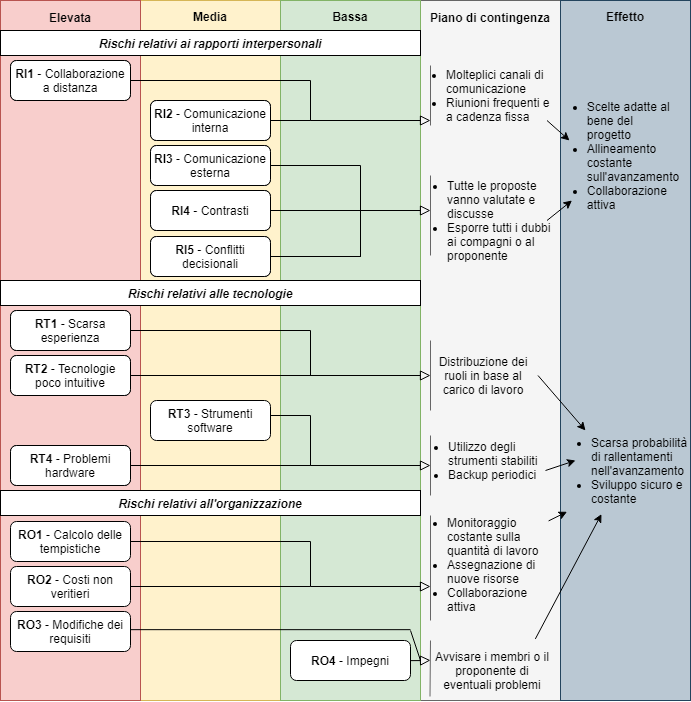
\includegraphics[width=17.5cm]{Images/rischi}
\caption{Attività di contingenza}
\end{figure}


